
\chapter{Ergebnis der Anforderungsumsetzung}\label{ch:ergebnis}

\vspace{5mm}
\begin{displayquote}
    The chief difficulty Alice found at first was in managing her flamingo.
    \par\hfill\cite{Car65}
\end{displayquote}
\vspace{25mm}

Die in der Einleitung dieses Dokuments formulierten Anforderungen (siehe Abschnitt~\ref{sec:einleitung}) wurden mit Meilenstein 5 in der \textit{Scoring Demo} umgesetzt, abgesehen von den grafischen Effekten, die das \textit{Game Feel} aufwerten sollten.

Im Folgenden geben wir einen Überblick über die Umsetzung des Spielkonzeptes und der Lastkriterien, die wir als Kernanforderung verstehen.

\subsection*{Umgesetztes Spielkonzept}
Die \textit{Scoring Demo} zählt nach dem Start des Spiels einen Countdown von 3 Minuten herunter.
Der Spieler beginnt mit 3 Leben und muss in dieser Zeit versuchen, einen möglichst hohen Punktestand zu erreichen.
Hierbei besteht die Schwierigkeit nicht bloss darin, sich geschickt einen Pfad durch die Gegnerwellen zu bahnen, sondern wird durch verschiedene physikalische Effekte der Schiffsteuerung erschwert: Die Geschwindigkeit beeinflusst in Zusammenhang mit der Masse des Schiffs die Manövierfähigkeit, so dass Richungswechsel einer gewissen vorausschauenden Planung bedürfen.
In diesem Zusammenhang wurde die Kamera entgegen einer fürhenren Phase nicht mehr an den Spieler gekoppelt, sondern beobachtet jetzt statisch die Spielwelt von oben, um die durch die Trägsheitmomente des PSielerschiffs erschwerte Steuerung zu kompensieren.
Damit ist die Umsetzung der \textit{Scoring Demo} näher an dem ersten Teil der Geometry Wars-Reihe, bei der die Kamera ebenfalls statisch über dem Spielfeld positioniert ist (siehe Abbildung~\ref{fig:geometrywars_pgr}.

\begin{figure}[!htbp]
    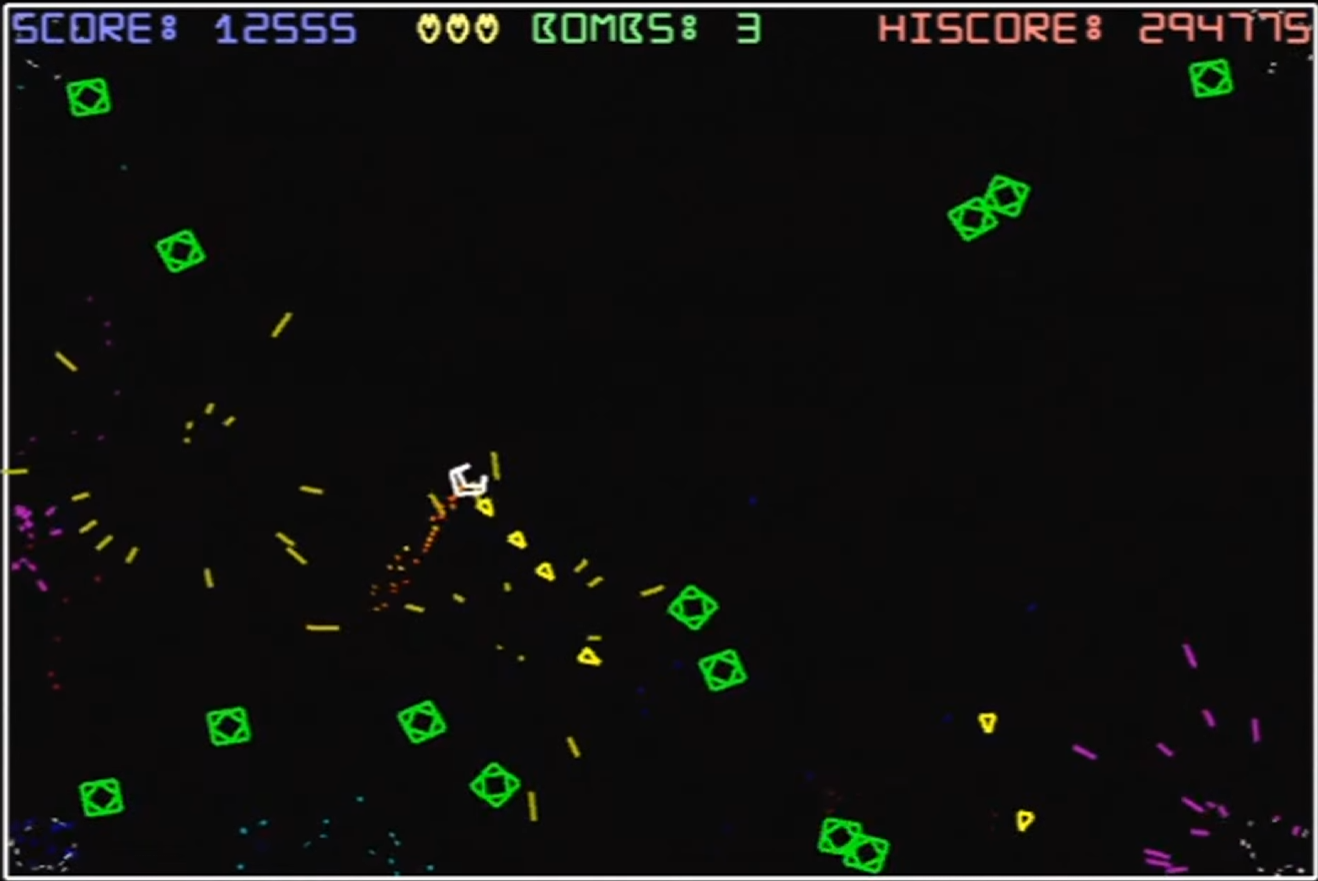
\includegraphics[width=\linewidth]{content/de/ergebnis/img/geometrywars_pgr}
    \caption{Ausschnitt einer Spielszene von \textit{Geometry Wars} als Minispiel in \textit{Project Gotham Racing 2}. (Quelle: \url{https://www.youtube.com/watch?v=KSoyRPQ1DjQ)} (abgerufen am 28.03.2026))}
    \label{fig:geometrywars_pgr}
\end{figure}




Durch die Verwendung eines identischen Seeds bei jedem Lauf  erhält der Spieler aber die Möglichkeit, die Spawnwellen der Gegner zu lernen und sich so auf die Herausforderung einzustellen.\\

Ist die Zeit abgelaufen, endet das Spiel.
Der Spieler erhält die Möglichkeit, das Spiel zu beenden und in den Titelbildschirm zurückzukehren, oder den Lauf zur wiederholen.
Gleiches gilt für den Fall, dass der Spieler alle Leben verliert.

\subsection*{Umgesetzte Lastkriterien}
Die Anforderungen bezüglich der Lastkriterien wurden im ursprünglichen Dokument eher allgemein formuliert und haben mit dem Kriterium ``Stabile Framerate von mindestens 60 FPS bei gleichzeitiger Darstellung von über hundert Gegnern und Objekten'' viel Spielraum bei der Umsetzung gelassen.

Die Anforderungen konnten auf den Testsystemen erfüllt werden (siege Abbildung~\ref{fig:lastkriterien}).
Zur Validierung erfolgte mit Meilenstein 5 die Umsetzung der \textit{Runtime Test Demo}, die einen spezieleln Bildausschnitt darstellt: Über einen vorkunfigurierten \textit{GameObject}-Pool mit einer Größe von $10,000$ Objekten kann über einen Schieberegler die Anzahl der gleichzeitig darzustellenden Objekte ausgewählt werden. Die Objekte werden über den \texttt{RandomSpawnPlacer} und \texttt{MoveInitializer} aus dem \texttt{spawn}-Modul mit zufälliger Platzierung und Bewegungsrichtung initialisiert.
Auf dem leistungsfähigen Testsystem (AMD Ryzen 9 9950X3D, 64\,GB RAM, Asus ROG Astral GeForce 5090 RTX) konnten Framerateeinbrüche auf unter 60 FPS ab ca $1600$ Spielobjekten festgestellt werden.
Hierbei uist zu beacchten, dass Optimierungen der Engine hauptsächlich CPU-seitig durch die in Abschnitt~\ref{sec:ecs} beschriebene ECS-Architektur ansetzen, und keine Optimierungen hinsichtlich der GPU-Auslastung erfolgen: Es findet kein GPU-Instanceing statt, stattdessen werden für alle $N$ dargestellten Spielobjekte auch $N$ Draw Calls ausgeführt.
Dies wird als \textit{draw call bound} bezeichnet und beschreibt, wie die Ansteuerung des Grafik-Backends (hier: OpenGL) zum Flaschenhals wird, noch bevor die GPU ausgelastet ist.
Außerdem werden die \textit{Uniform Values} bei jedem \textit{Draw Call} gesetzt, auch hier bietet sich Optimierungspotenzial an, da einige Werte pro Frame global wiederverwendet werden können.

\subsection*{Aufwertung des GameFeels durch grafische Effekte}
Mit der Konzentration auf die Umsetzung der Kernmechaniken und -features wurde die Anforderung zur Aufwertung des \textit{Game Feels} durch grafische Effekte nicht umgesetzt.
Hier bieten sich verschiedene Möglichkeiten an, wie beispielsweise der Einsatz von Partikeleffekten bei Explosionen und einer Veerformung des Grids bei Kollisionen, um die Auswirkungen der Spielmechaniken auf die Spielwelt zu visualisieren.


\begin{figure}[!htbp]
    \centering

    \begin{subfigure}{0.48\columnwidth}
        \centering
        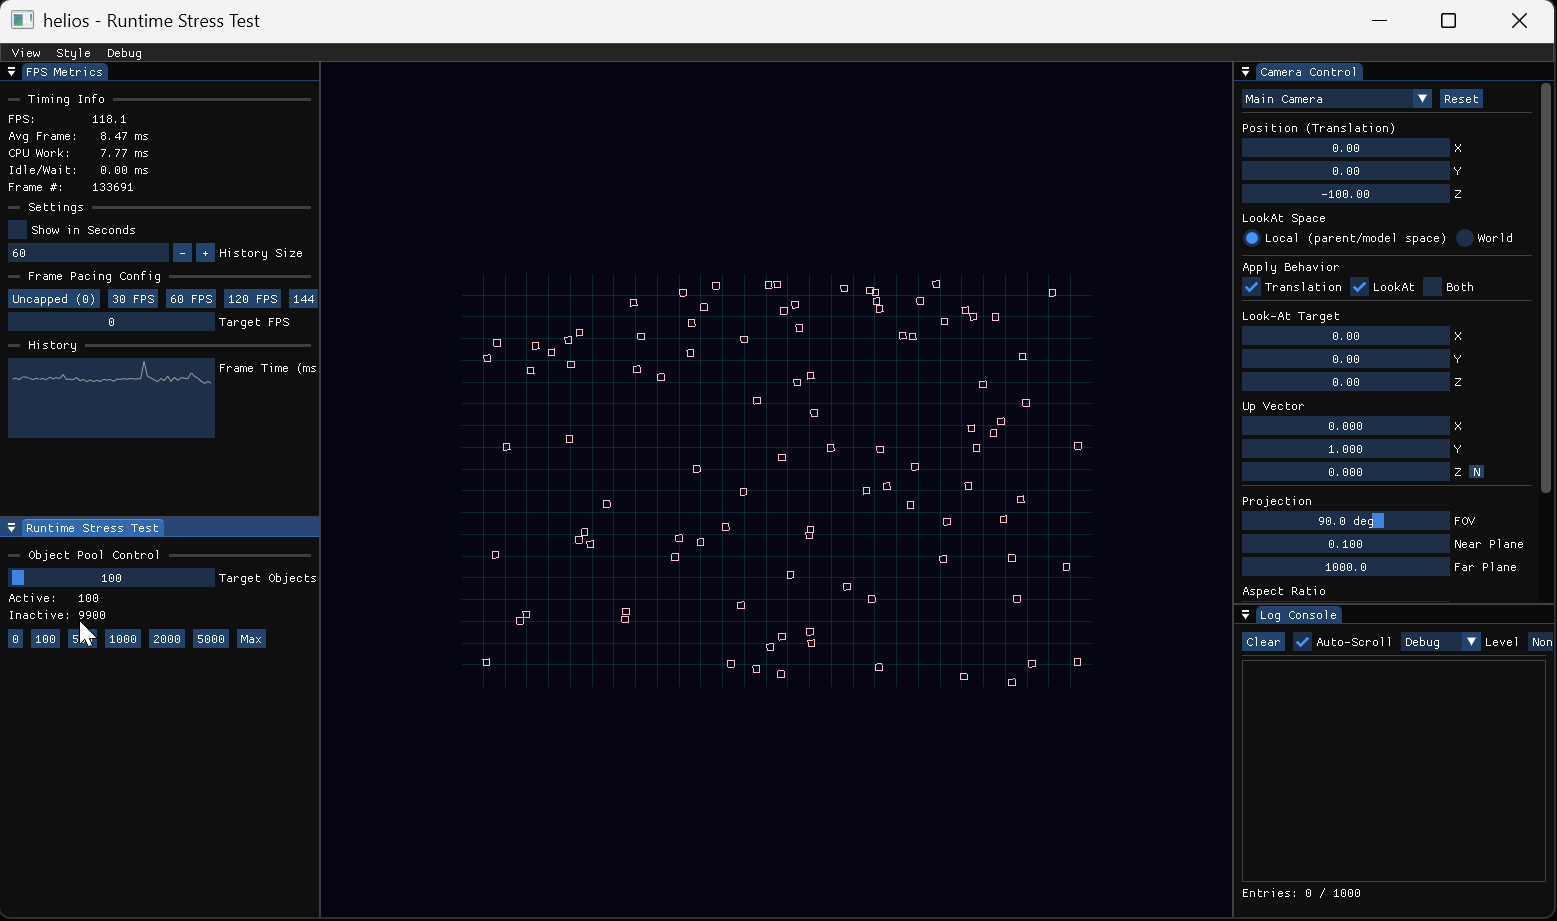
\includegraphics[width=\linewidth]{content/de/ergebnis/img/go100}
    \end{subfigure}
    \hfill
    \begin{subfigure}{0.48\columnwidth}
        \centering
        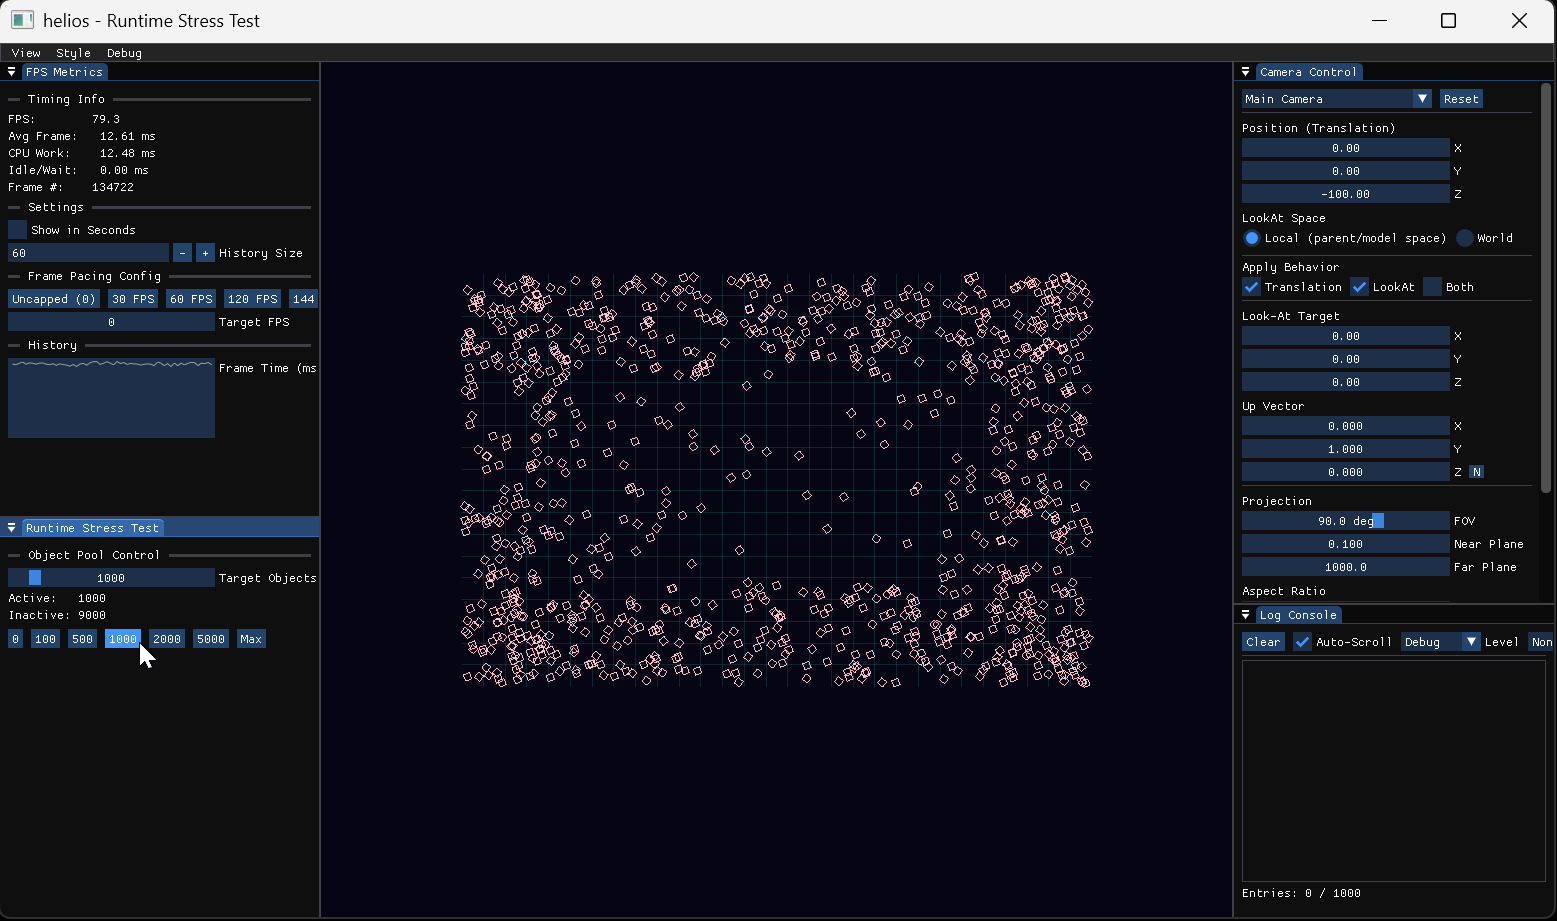
\includegraphics[width=\linewidth]{content/de/ergebnis/img/go1000}
    \end{subfigure}

    \vspace{2mm}

    \begin{subfigure}{0.48\columnwidth}
        \centering
        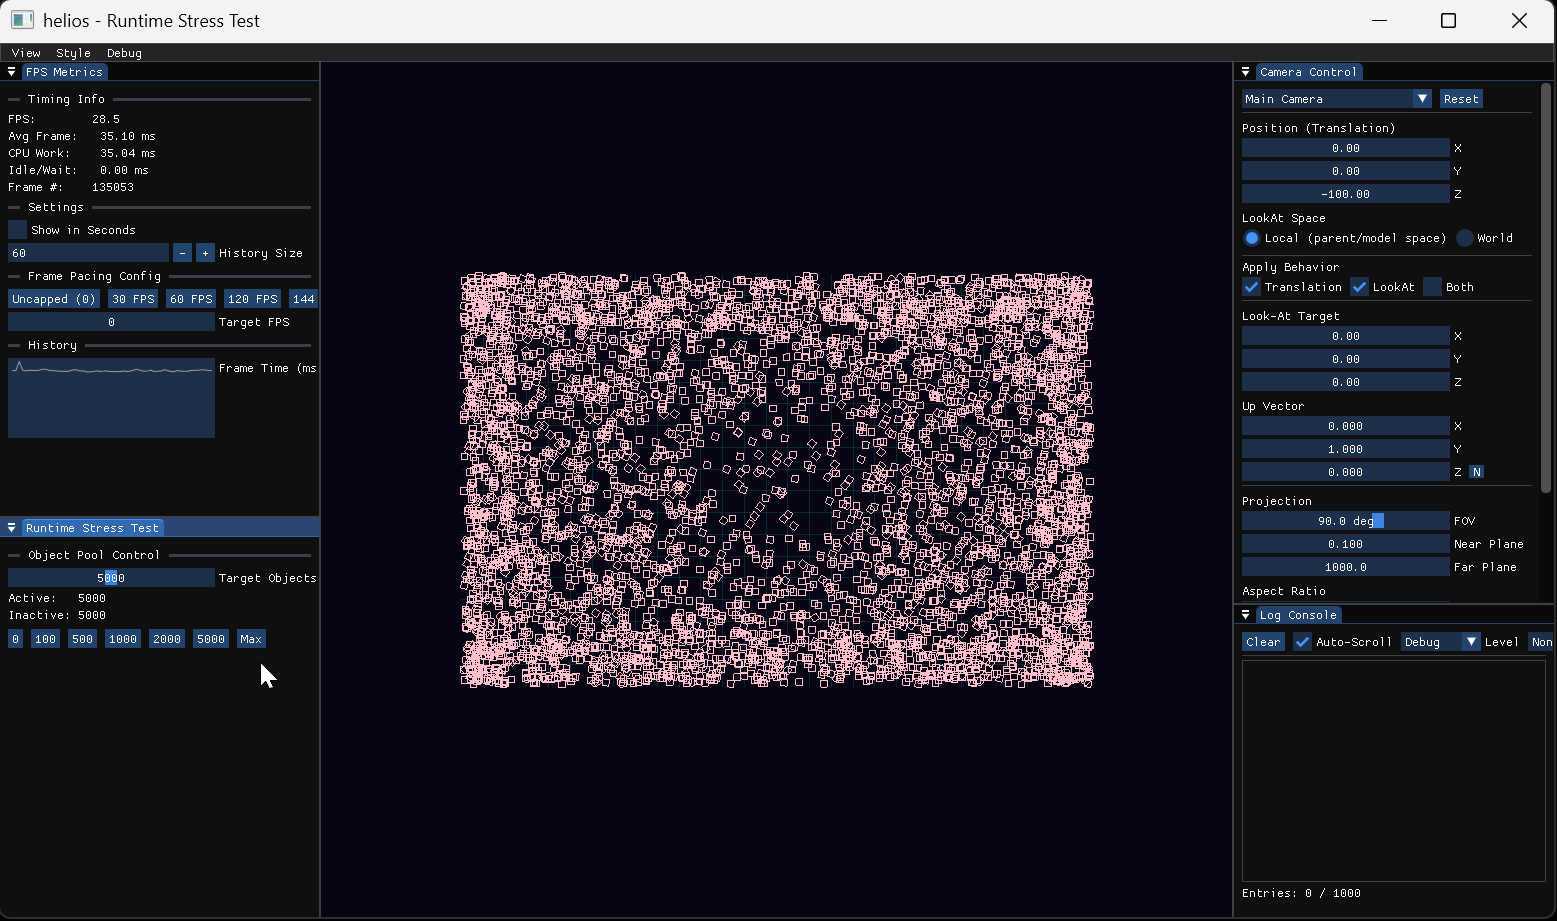
\includegraphics[width=\linewidth]{content/de/ergebnis/img/go5000}
    \end{subfigure}
    \hfill
    \begin{subfigure}{0.48\columnwidth}
        \centering
        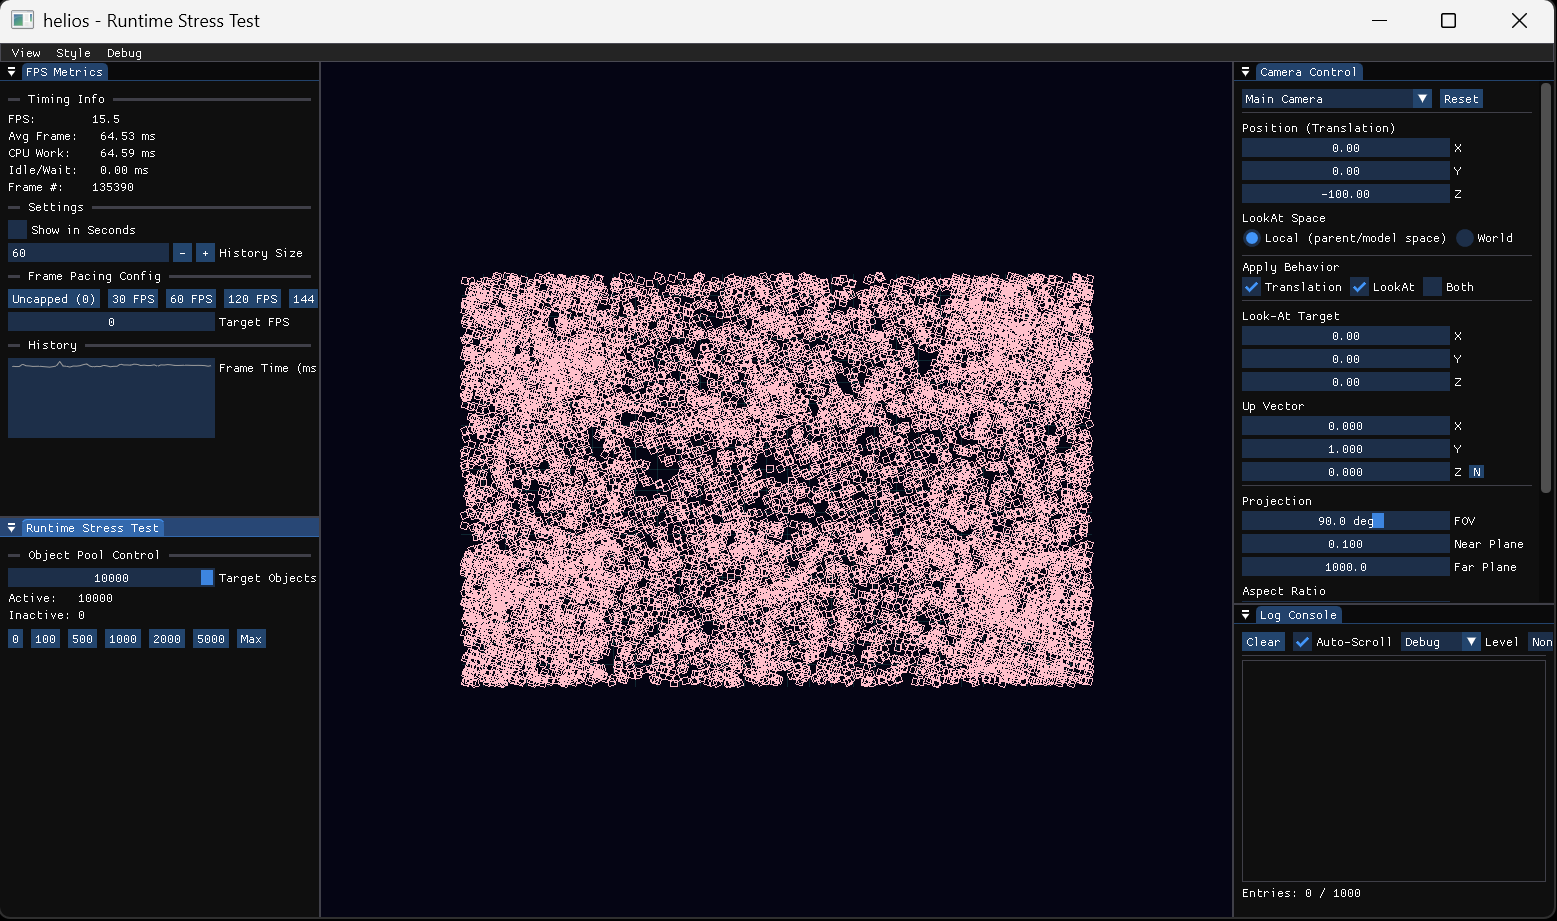
\includegraphics[width=\linewidth]{content/de/ergebnis/img/go10000}
    \end{subfigure}

    \caption{Darstellung einer unterschiedlichen Anzahl von Spielobjekten und ihre Auswirkung auf die Performance. Bei 100 Objekten läuft die \textur{Runtime Test Demo} stabil bei der durch die von der Bildwiederholfrequenz des Monitors vorgegebenen 120 fps. Bei 1000 Objekten pendelt sich die Framerate bei ungefähr $80$ fps ein, bei 5000 liegt sie bei ca. $30$ fps. Bei $10,000$ Objekten liegt sie bei noch ca. 15 fps (von oben links im Uhrzeigersinn). Es ist also eine stabile Skalierung bemerkbar, die wir auf die Optimierungen durch die ECS-Architektur zurückführen. Optimierungen der Rendering-Pipeline, um Spiele in einem Kontext von $10,000$ gleichzeitig darzustellenden Objekten zu untersützen, wären also zwingend notwendig. (Quelle: eigene Aufnahme)}
    \label{fig:lastkriterien}
\end{figure}
